\chapter{The Transformer Block}

\section{Architecture Overview}
The `pure_transformer` uses a standard "Pre-Norm" architecture, which is more stable for training deep networks than the original Post-Norm design.

Each block consists of two sub-layers:
\begin{enumerate}
    \item Assessment (Attention): \textit{"What other tokens are relevant to me?"}
    \item Processing (Feed-Forward): \textit{"What does this mean?"}
\end{enumerate}

\begin{figure}[H]
    \centering
    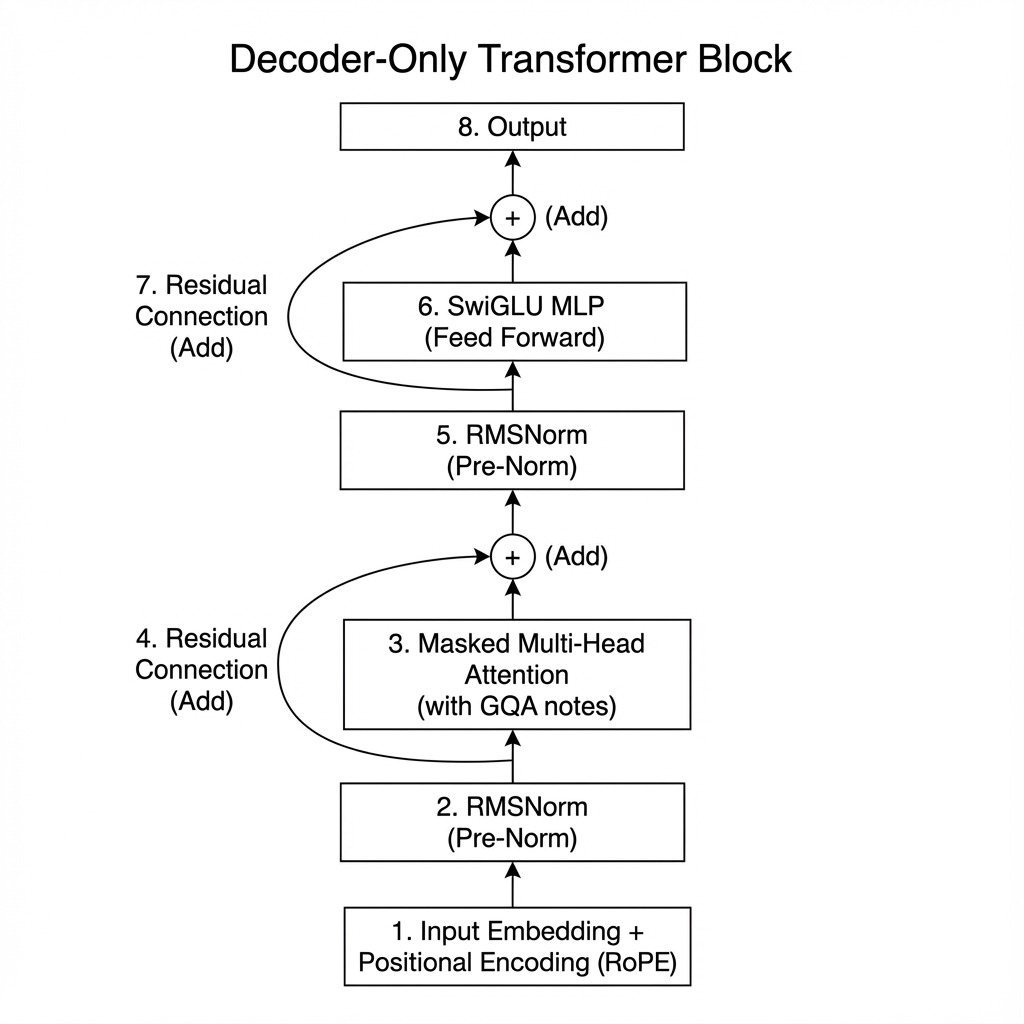
\includegraphics[width=0.6\textwidth]{images/transformer_architecture.png}
    \caption{Decoder-Only Transformer Block Structure}
    \label{fig:transformer_block}
\end{figure}

\begin{lstlisting}[language=Python, caption=TransformerBlock Forward Pass]
# model/transformer.py

def forward(self, x, cos, sin, attention_mask=None, kv_cache=None):
    # 1. Attention with Residual
    # Note: Norm is applied BEFORE attention (Pre-Norm)
    h, new_kv = self.attention(
        self.input_norm(x), cos, sin, attention_mask, kv_cache
    )
    x = x + h  # Residual connection
    
    # 2. MLP with Residual
    # Note: Norm is applied BEFORE MLP
    x = x + self.mlp(self.post_attn_norm(x))
    
    return x, new_kv
\end{lstlisting}

\section{Normalization: RMSNorm}
We use \textbf{RMSNorm} (Root Mean Square Normalization) instead of LayerNorm. RMSNorm is computationally cheaper (no mean subtraction) and equally effective.

\begin{lstlisting}[language=Python, caption=RMSNorm Implementation]
# model/transformer.py

def rms_norm_func(x: Tensor, normalized_shape: Tuple[int, ...], 
                  weight: Optional[Tensor] = None, eps: float = 1e-6) -> Tensor:
    """RMSNorm using standard PyTorch ops."""
    variance = x.pow(2).mean(-1, keepdim=True)
    x_normed = x * torch.rsqrt(variance + eps)
    if weight is not None:
        x_normed = x_normed * weight
    return x_normed
\end{lstlisting}

\section{Feed-Forward Network: SwiGLU}
The Feed-Forward Network (FFN) is where the model stores "knowledge". We use the \textbf{SwiGLU} variant, which has been shown to perform better than standard ReLU or GELU MLPs (used in Llama, PaLM).

It involves three linear projections instead of two:
$$ \text{SwiGLU}(x) = (\text{SiLU}(xW_g) \odot xW_u)W_d $$

\begin{lstlisting}[language=Python, caption=SwiGLU MLP]
# model/transformer.py

class SwiGLUMLP(nn.Module):
    def __init__(self, hidden_size: int, intermediate_size: int, dropout: float = 0.0):
        super().__init__()
        # Three projections
        self.gate_proj = nn.Linear(hidden_size, intermediate_size, bias=False)
        self.up_proj = nn.Linear(hidden_size, intermediate_size, bias=False)
        self.down_proj = nn.Linear(intermediate_size, hidden_size, bias=False)
        
    def forward(self, x: Tensor) -> Tensor:
        # SiLU(Gate) * Up -> Down
        return self.down_proj(F.silu(self.gate_proj(x)) * self.up_proj(x))
\end{lstlisting}
